\documentclass{article}
\usepackage[utf8]{inputenc}
\usepackage[frenchb]{babel}
\usepackage[T1]{fontenc}
\usepackage{graphicx}

\setlength{\oddsidemargin}{0pt} % Marge gauche sur pages impaires
\setlength{\evensidemargin}{9pt} % Marge gauche sur pages paires
\setlength{\marginparwidth}{54pt} % Largeur de note dans la marge
\setlength{\textwidth}{481pt} % Largeur de la zone de texte (17cm)
\setlength{\voffset}{-18pt} % Bon pour DOS
\setlength{\marginparsep}{7pt} % Séparation de la marge
\setlength{\topmargin}{0pt} % Pas de marge en haut
\setlength{\headheight}{13pt} % Haut de page
\setlength{\headsep}{10pt} % Entre le haut de page et le texte
\setlength{\footskip}{27pt} % Bas de page + séparation
\setlength{\textheight}{708pt} % Hauteur de la zone de texte (25cm)

\title{Rapport de Réseaux et Télécoms \\ Séance de TP 1}
\author{Florian Delavernhe et Thomas Minier \\ groupe 501A}
\date{Jeudi 29 Janvier 2014}

\begin{document}

\maketitle
\vspace{5cm}
\tableofcontents
\newpage

\section{Introduction}

Durant cette séance de travaux pratiques, le but était de connecter notre machine à un réseau local, de la configurer, puis de configurer une passerelle et d'établir une route entre deux réseaux locaux via cette dernière. Ce rapport contient notre démarche, nos observations et le résultat de nos travaux.

\section{Configuration de la machine}

Avant toute chose, nous avons coupé le manager réseau de la machine, pour pouvoir configurer la carte réseau manuellement. Pour cela, nous avons utilisé la commande suivante :
\begin{verbatim}
/etc/init.d/network-manager stop
\end{verbatim}

Nous avons ensuite relier notre machine à un switch via un câble ethernet. Ce switch étant relié à tous les ordinateurs, il crée un sous-réseau local. Puis, nous avons configuré notre machine pour lui assigner une adresse IP.

Pour ce faire, nous avons utilisé la commande \textbf{ifconfig}. Notre machine ayant le numéro 4 et étant situé dans le sous-réseau 0, nous avons utiliser l'adresse 192.168.0.4 pour identifier notre machine. Il s'agit d'une adresse de classe C, son netmask est donc 255.255.255.0 . La commande reconnaissant intuitivement le netmask, ce dernier est donc optionnel. \textbf{eth0} représente la carte réseau numéro 0 de la machine. La commande complète que nous avons utilisé est la suivante :
\begin{verbatim}
ifconfig eth0 192.168.0.4 netmask 255.255.255.0
\end{verbatim}

Pour tester la connexion au sous-réseau local, nous avons essayé d'envoyer un message à une autre machine du sous-réseau via la commande \textbf{ping}. Nous avons choisi la machine numéro 5, qui a donc comme adresse IP 192.168.0.5 . Nous n'envoyons que 5 messages, via l'option \textbf{-c}, pour éviter de surcharger les logs réseaux. La commande complète est la suivante :
\begin{verbatim}
ping -c 5 192.168.0.5
\end{verbatim}
Cette commande nous a affiché une ligne par message, avec le format suivant :
\begin{verbatim}
64 bytes from 192.168.0.4 req=0 time:1.38ms
\end{verbatim}
Par rapport au premier message, le temps de réponse a diminué, affichant une moyenne de 0.759ms. Nous pensons que cela est dû au fait que la machine a déjà établi une connexion avec l'autre machine et connaît déjà le chemin. En effet, lors de l'envoi du premier message, le switch transmet le message à toutes les machines du sous-réseau, et seule celle a qui le message est destiné le lit.

A la fin de l'envoi, le terminal nous affiche le message suivant :
\begin{verbatim}
5 packets transmis, 5 reçus, 0% loss
\end{verbatim}

\section{Configuration de la passerelle}

Nous avons ensuite tenté de connecter les deux sous-réseaux, respectivement de numéro 0 et 1. Pour ce faire, nous avons commencé par connecter notre switch à la passerelle avec un câble ethernet. Ensuite, nous avons configuré l'adresse IP de la passerelle. \\

Tout d'abord, nous avons tapé la commande suivante pour passer la machine en mode passerelle :
\begin{verbatim}
echo 1 > /proc/sys/net/ipv4/ip_forward
\end{verbatim}
\newpage

Ensuite, nous avons configuré les adresses IP des sous-réseaux 0 et 1. Le câble relié au sous-réseau 0 est connecté à la carte réseau numéro 0, nous utiliserons donc \textbf{eth0}, et le câble relié au sous-réseau numéro 1 est connecté à la carte réseau numéro 1, nous utiliserons donc \textbf{eth1}.
De plus, l'adresse IP réservée pour le sous-réseau 0 sera 192.168.0.254, et celle réservée au sous-réseau 1 sera 192.168.1.254. Ces adresses sont de classes C et ont donc comme netmask 255.255.255.0 . Nous avons utilisé les commandes suivantes :
\begin{verbatim}
ifconfig eth0 192.168.0.254 netmask 255.255.255.0
ifconfig eth1 192.168.1.254 netmask 255.255.255.0
\end{verbatim}

Pour vérifier que notre passerelle était bien configurée, nous avons utilisée la commande \textbf{ping}. La passerelle ayant l'adresse 192.168.0.254 de notre côté, nous avons utilisé la commande suivante pour lui envoyer quelques messages :
\begin{verbatim}
ping -c 5 192.168.0.254
\end{verbatim}
La réponse nous a certifiée que la connexion était bien établie.

\section{Établissement d'une route vers la passerelle}

Une fois la passerelle configurée, nous avons du établir une route entre notre ordinateur et la passerelle. cela nous permettra d'accéder à l'autre sous-réseau. Pour ce faire, nous avons utilisé la commande \textbf{route}. L'adresse IP du sous-réseau vers lequel nous voulons établir une route est 192.168.1.0 . Il s'agit d'une adresse de classe C, son netmask vaut donc 255.255.255.0 . La passerelle qui va nous permettre de nous connecter à ce sous-réseau à elle l'adresse 192.168.0.254 . Il s'agit de l'adresse de la passerelle de notre côté. Nous avons utilisé la commande suivante :
\begin{verbatim}
route add -net 192.168.1.0 netmask 255.255.255.0 gw 192.168.0.254
\end{verbatim}

Pour tester que notre route a bien été établie, nous avons essayé d'envoyer des messages à une machine de l'autre sous-réseau avec la commande \textbf{ping}. Nous avons choisi la machine numéro 11, dont l'adresse IP est 192.168.1.11 . Nous avons utilisé la commande suivante :
\begin{verbatim}
ping -c 5 192.168.1.11
\end{verbatim}
La réponse nous a certifiée que la connexion était bien établie.

\section{Annexe : schéma du réseau local}

\begin{figure}[h]
\centering
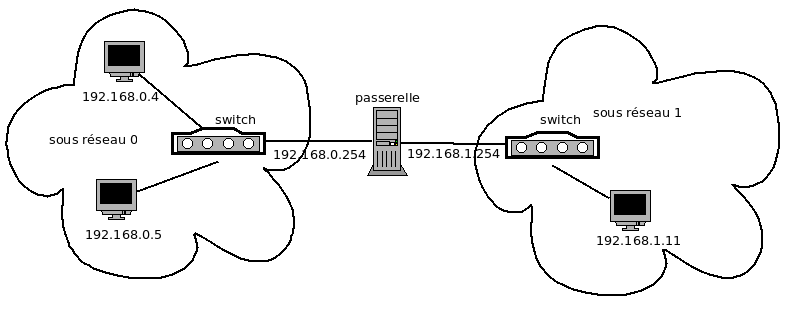
\includegraphics[scale=0.6]{reseau-tp1.png}
\caption{Représentation du réseau local}
\end{figure}

\end{document}
